\section{The IBL commissioning}\label{sec:IBL_commissioning}
%\pagestyle{plain}
\subsection{The IBL on surface commissioning}
%
The IBL detector went through a on surface commissioning, which consisted of two main parts: the commissioning of the services and a further test of the staves after the loading around the IPT.\\
A system test with two production staves of the IBL detector was performed in order to have a realistic estimation of the detector behavior in operation. A setup consisting of all detector services was installed in a cleanroom facility, replicating on-surface the powering chain. Production and pre-production parts were used. Functionality tests of the modules loaded on the staves were performed, in particular measurements of the detector performance with radioactive sources and data taking with cosmic rays.\\
Prior to loading around the IST, each of the 14 selected staves was tested by the so-called connectivity test. This was done to verify the electrical and functional integrity of the stave components after integration onto the IPT.


\subsubsection{The IBL system test}
%
\begin{figure}
\includegraphics[width=1.0\textwidth]{Images/IBL_paper/chapter08_Commissioning/IBL_connectivity.png}
\caption{Scheme of the IBL connectivity}
\label{fig:ibl_conn}
\end{figure}
Aim of the system test was to test the full IBL readout chain before the  insertion. For this purpose functionality test and data-taking were performed mounting two staves around the IPT support. For this setup the two staves that were damaged during the stave QA were used, stave 7 (ST07) and 8 (ST08). Those staves were rejected for the insertion at the QA because of the accident described in the previous Chapter. Nevertheless those were still partially functional and they suited good for the testing purpose of the setup. Additionally a thorough replacement of the wire-bonds was performed before the test. All services connected to the staves were production parts in order to have a realistic model of the final system as in ATLAS. Differently from the real data-taking the test used RCE based readout system.\\
The IBL connectivity consisted of several cables and patch panels, as schematized in the \reffigure~\ref{fig:ibl_conn}, where patch panels were dedicated boards that rearranged the cables wrapping and in which interlocks and regulators can be embedded.
Each stave was connected to the electrical services through the End of Stave cards (EoS), located at the first patch panel (PP0). Two cables exited the PP0, a 5 meter electrical cable with the FE-I4 communication and a 3.5 meter cable which took care of the Humidity and NTC information.\\
The first cable delivered the data, the clock and the command lines of the FE-I4 chips to the boards that took care of the electrical-to-optical signal conversion, the opto-boards. These opto-boards were located in a dedicated rack, the opto-box, which took care of the cooling of the opto-boards and their powering as well. From the opto-box 80 meters long optical fibers were connected to the readout system. LV control lines were as well connected either to the second patch panel (PP2) or to the final one (PP4).\\
The second cable took care of the NTC and humidity sensors located in the stave volume, feeding an Axon Connector which took care of the wrapping of the lines coming from the stave flex and the ones associated to environmental measurements. The HV, LV and sensors line were then connected into PP2. At this stage LV lines went through regulators, to minimize the voltage drop. PP2 is crucial for the IBL monitoring, because is the closest stage to the detector in which detector monitoring can happen.\\
From PP2 all the electrical cables are connected to PP4, where all the power supply and the interlock system for the HV are.\\
As a first step in the commissioning of the setup, a complete test of the electrical services was carried-out. This was performed by using a stave dummy load, a test board to mimic the stave power consumption and allows probing of all inputs and outputs, which was connected to PP0. This test was essential for the development of the final protocol for the commissioning of the services for both the system test and the final detector installed in the experiment.\\
The same CO$_{2}$ cooling as the stave QA was used in the system test. Temperature measurements at different supply voltage and module configurations were carried-out in order to simulate the power consumption expected during the detector lifetime.\\
Several measurements of the analogue performance of the modules were performed during the system test: first, test with existing configuration from the stave QA and then with configuration retuned at the same threshold target of \SI{1500}{\e} by the system test. The main difference between the two test-stands (QA and system test) was just in the service chain.
Figures \ref{fig:thresholdfinaltest7}-\ref{fig:totfinaltest8} compare the threshold values and ToT values obtained in the system test and during QA.
%%%%%%
\begin{figure}
                \centering
       	\null \hfill
               \subfloat[]{\label{fig:thresholdfinaltest7} \includegraphics[width=0.49\textwidth]{Images/IBL_paper/chapter08_Commissioning/thr7.png}}
        \hfill               
                \subfloat[ ]{\label{fig:thresholdfinaltest8} \includegraphics[width=0.49\textwidth]{Images/IBL_paper/chapter08_Commissioning/thr8.png}}
        \hfill \null
        
        \null \hfill
               
                \subfloat[ ]{\label{fig:noisefinaltest7} \includegraphics[width=0.49\textwidth]{Images/IBL_paper/chapter08_Commissioning/noise7.png}}
        \hfill
                \subfloat[ ]{\label{fig:noisefinaltest8} \includegraphics[width=0.49\textwidth]{Images/IBL_paper/chapter08_Commissioning/noisethr8.png}}
        \hfill \null
        
        \null \hfill
        \subfloat[]{\label{fig:totfinaltest7} \includegraphics[width=0.49\textwidth]{Images/IBL_paper/chapter08_Commissioning/tot7.png}}       
        \hfill
        \subfloat[]{\label{fig:totfinaltest8}\includegraphics[width=0.49\textwidth]{Images/IBL_paper/chapter08_Commissioning/tot8.png}}
       \hfill \null   
        \caption{Stave ST07 (left) and ST08 (right) Threshold (a,b), Noise (c,d)  and ToT (e,f) results. It should be noted that on ST07 the front-end chip A2-1 was not working due to a short between Reset and GND pads and on ST08 A8-1 the front-end chips A8-1 and C5-2 were not working due to broken power regulators. Therefore, they were disabled during the system test operation and only QA data are shown for them in the comparison plots. }
\end{figure}

%\begin{figure}
%                \centering
%        
%                \subfloat[ \label{fig:sourcescanfinaltest7}]{\includegraphics[width=0.5\textwidth]{Images/IBL_paper/chapter08_Commissioning/source7.png}}
%                \subfloat[\label{fig:sourcescanfinaltest8}]{\includegraphics[width=0.5\textwidth]{Images/IBL_paper/chapter08_Commissioning/sourcescanst8.png}}\\
%                \subfloat[\label{fig:cosmic}]{\includegraphics[width=0.5\columnwidth]{Images/IBL_paper/chapter08_Commissioning/cosmic.png}}
%                       \caption{Source scans with $^{241}$Am and $^{90}$Sr for stave ST07 (a) and ST08 (b). A cosmic ray passing through a module of stave ST07. (c)}
%\end{figure}

%%%%%%
In Figure \ref{fig:noisefinaltest7} and \ref{fig:noisefinaltest8} the threshold noise distributions of both staves are showed. It can be seen that the noise is low except for two modules that are neighboring the broken ones. The results obtained for different tunings showed excellent performance with a slightly lower and more homogeneous noise level compared to the QA, as a more sophisticated powering and grounding schema is used in the system test.\\
A noise scan was performed directly after tuning, after several steps of noisy pixel masking and while running a threshold scan simultaneously on the other stave. The results show no increased noise on ST07 while a scan was running on ST08. This test confirmed that no crosstalk happened at the service level in two neighboring staves.\\
%Source scans were performed with $^{241}$Am and $^{90}$Sr and the results shown in Figure~\ref{fig:sourcescanfinaltest7} and \ref{fig:sourcescanfinaltest8} have been obtained after one hour of data-taking. The white areas correspond to the disabled modules and the blue shade visible from left to right on ST07 can be identified as the cooling tube. In addition, cosmic data was successfully taken for two hours and Figure \ref{fig:cosmic} shows a cosmic ray passing through a module of ST07.\\
The system test was also used to confirm functionality of the interlock system. Both showed no problems during the complete duration of the system test.\\
%

\subsubsection{The IBL connectivity test}
\begin{figure}
\centering
\subfloat[\label{fig:threshold}]{\includegraphics[width=0.49\textwidth]{Images/IBL_paper/chapter08_Commissioning/econ_res_threshold.png}}
\subfloat[\label{fig:noise}]{\includegraphics[width=0.49\textwidth]{Images/IBL_paper/chapter08_Commissioning/econ_res_noise.png}}\\
\subfloat[\label{fig:tot}]{\includegraphics[width=0.49\textwidth]{Images/IBL_paper/chapter08_Commissioning/econ_res_tot.png}}
 \caption{Average and RMS of the chip-to-chip Front-End (FE) threshold \subref{fig:threshold}, noise \subref{fig:noise} and ToT \subref{fig:tot} difference between the obtained results with the Connectivity Test minus the quality-assurance (QA) values for the 14 integrated staves after integration around the Inner Positioning Tube (IPT). Data Taking was performed using the quality-assurance configuration file targeted to \SI{3000}{\e} and 10 ToT at \SI{16}{\kilo\e}. Maximum and minimum FE threshold mean values of the 14 staves are represented for each chip position by the filled area.}
\end{figure}

The purpose of the stave connectivity test was to verify the electrical and functional integrity of each staves after its integration onto the IPT and test of the services chain. Once a stave was integrated onto the IPT two sets of the electrical and functional tests have been performed: one right after the stave integration and one just after having integrated its neighbor. In both cases, the test results were directly compared to the stave QA measurements.\\
Similarly to the stave QA, the readout system of the connectivity test was based on the RCE system. The front-end chips and sensors were powered by commercial and portable power-supplies, while the temperature of the environment and modules and humidity were read out by a dedicated DCS system with an interlock on the LV power-supplies for the module temperature higher than \SI{30}{\celsius}. All the connectivity test components were housed into a mobile rack for allowing easy movement of the system around the IBL package.\\
Since the integrated staves were not cooled, all the scans needed to check the electrical and functional integrity were performed in a very short time (\SI{10}{\second} maximum) to prevent module-temperatures higher than \SI{30}{\celsius}. For that purpose, the read-out system and the LV power-supply were operated by using fully automatic processes in order to minimise the time of the LV powering. \\
The connectivity test-list consists in:
\begin{itemize}
 \item Digital- and Analog-tests and read-out check of the front-end register values for checking the front-end functionality;
 \item Threshold scan without powering the sensor bias voltages for looking for disconnected bumps between the sensor and front-end;
 \item I-V sensor measurements for cross-checking the sensor voltage breakdown;
 \item Digital- and Analog-tests, Threshold- and ToT-scans with biased sensors for cross-checking the stave quality.
\end{itemize}
For operations at temperature lower than \SI{30}{\celsius}, threshold and ToT scans were performed with only \SI{16}{\percent} of the front-end channels on.\\
Figure \ref{fig:threshold}, \ref{fig:noise} and \ref{fig:tot} show the comparison of the results of the threshold, noise and ToT values between the stave QA and connectivity test. The plots show the difference between the connectivity test and QA results. Since cooling was not operated during the connectivity test, the noise and threshold values are larger in the connectivity test than the stave QA. Especially, the modules with the 3D sensors are more sensitive to the difference in temperature than the planar sensors. These deviations were not an issue since they were within expected level. Furthermore, no significant change of the performance was observed in the other scans.\\
Together with the electrical performance, the connectivity test also revealed hardware problems, such as the disconnection of a wire and a broken NTC in the type-I cable and the merged solder with the neighboring lines in the intermediate flex. They were fixed soon after the problems were found except for the broken NTC which was difficult to access after closing the IBL with the dummy IST, and was therefore decided to leave un-repaired.


%\begin{figure}
%\begin{center}
%\includegraphics[width=0.5\columnwidth]{Images/IBL_paper/chapter08_Commissioning/econ_res_noise.png}
%\end{center}
%\caption{Average and RMS of the chip-to-chip Front-End (FE) noise difference between the obtained results with the Connectivity Test minus the quality-assurance (QA) values for the 14 integrated staves after integration around the IPT (IBL positioning tube). Data Taking was performed using the QA configuration file targeted to \SI{3000}{\e} and 10 ToT at \SI{16}{\kilo\e}. Maximum and minimum FE noise mean values of the 14 staves are represented for each chip position by the filled area (most four outer chips per side, using 3D sensor technology, shown different noise behaviour).}
%\label{fig:noise}
%\end{figure}


%\begin{figure}
%\begin{center}
%\includegraphics[width=0.5\columnwidth]{Images/IBL_paper/chapter08_Commissioning/econ_res_tot.png}
%\end{center}
%\caption{Average and RMS of the chip-to-chip Front-End (FE) ToT mean values difference between the obtained results with the Connectivity Test minus the quality-assurance (QA) values for the 14 integrated staves after integration around the IBL Positioning Tube (IPT). Data Taking was performed using the QA configuration file targeted to \SI{3000}{\e} and 10 ToT at \SI{16}{\kilo\e}. Maximum and minimum FE ToT mean values of the 14 staves are represented for each chip position by the filled area. }
%\label{fig:tot}
%\end{figure} 

%\subsection{The IBL assembly electrical test}
%\subsection{The insertion}

%\subsection{Electrical test after the insertion}

\subsection{Detector calibration after the insertion}
In order to be ready for the data-taking period the IBL needed to went through a dedicated phase of calibration. This phase was divided in two main operation:
\begin{itemize}
\item the tuning of the front-end parameters related to the threshold and the Charge to ToT conversion;
\item the optimization of the timing response for each front end couple, needed for being as most efficient as possible in one single bunch crossing readout window.
\end{itemize}

%Given the strong connection of the front-end parameters, the two operations are tied together, but for simplicity they are treated separately in the following sections and the final results will be presented.

A description of the two calibrations follows.

\subsubsection{Charge calibration}

Given the effect of radiation damage the threshold and charge-to-ToT settings of the IBL needs to be constantly monitor and adjusted periodically in presence of beam. As discussed in Section~\ref{sec:rad_dam}, the maximum signal pulse height of a silicon sensors decrease with the luminosity, while the equivalent noise charge increases, so that the threshold will need to be lowered for keeping high efficiency performance of the IBL.\\
While lowering the threshold allows to detect low charge signals, it also increase the possibility that noise pass the discriminator and it is treated as a signal.
\begin{figure}
\centering
\includegraphics[width=0.6\textwidth]{Images/IBL_commissioning/occupancy_vs_threshold.png}
%\subfloat[]{\label{pic:anal_fei4}\includegraphics[width=0.5\textwidth]{Images/IBL_commissioning/fei4-scheme.png}}
\caption{Noise occupancy per pixel dependence on the FE-I4 threshold. The noise occupancy measured for PPS and 3D assemblies after irradiation to $5\times10^{15}~n_{eq}/cm^2$ and cooled to $-15^{\circ}C$. Dead pixels were excluded from the measurement. \cite{DavidPohl}}
\label{pic:noise_occupancy}
\end{figure}
Figure~\ref{pic:noise_occupancy} shows the noise occupancy per pixel for different threshold settings\cite{PohlLeon}. The measurement was done for the two different sensors technology: planar (PPS) and 3D sensors. The measurement was performed averaging over $3\times10^8$ triggers.\\
For the beginning of the data-taking a conservative value of 2500 electrons was chosen as target threshold, the value will be lowered with time as the integrated luminosity will increase.

%Given the new readout system developed for the IBL, discussed in Chapter~\ref{sec:ibl_daq}, all the tuning algorithm needed to be adapted to the new chip.


%The charge calibration tuning happens at the level of the analog circuitry of the FE-I4. A two-stage amplifier configuration is used, the first stage (Preamp) is a cascode amplifier while the second stage (Amp2) is a folded cascode AC coupled to the Preamp. The two-stage choice allows to provide enough gain before the discriminator while permitting the optimization in the choice of the preamp feedback capacitor ($C_{f1}$).

\begin{figure}
\centering
\null \hfill
\subfloat[]{\label{pic:vthin}\includegraphics[width=0.5\textwidth]{Images/IBL_commissioning/vthin.png}}
\hfill
\subfloat[]{\label{pic:prmpvbpf}\includegraphics[width=0.5\textwidth]{Images/IBL_commissioning/prmpvbpf.png}}
\hfill \null
\null \hfill
\subfloat[]{\label{pic:tdac}\includegraphics[width=0.5\textwidth]{Images/IBL_commissioning/tdac.png}}
\hfill
\subfloat[]{\label{pic:fdac}\includegraphics[width=0.5\textwidth]{Images/IBL_commissioning/fdac.png}}
\hfill \null
\caption{(a) Threshold as function of the global settings. (b) TOT response as function of the global feedback current. (c) Threshold as function of the pixel level threshold setting. (d) TOT response as a function of the pixel level feedback current setting.}
\end{figure}

%The discriminator is built with a two-input voltage comparator and a threshold voltage generator. Signal shaping is only done by the preamp with an adjustable return to the baseline, while the second stage provides only the voltage gain, given by the ratio $\frac{C_c}{C_{f2}}$. The return to the baseline and the discriminator threshold are individually adjustable in each pixel, with dedicated local and global pixel registers. Two selectable capacitors are provided for analog calibration injection.\\
%The preamp feedback has a low frequency active filter for DC leakage current compensation, and the amount of DC leakage is mirrored to a column-parallel output. The comparator output is fed to the digital pixel region
\begin{figure}
\centering
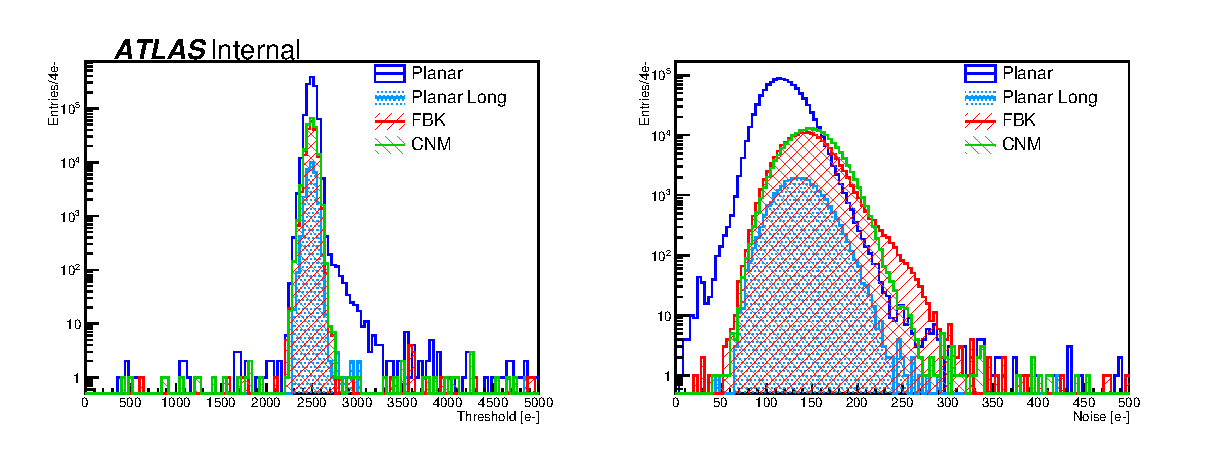
\includegraphics[width=1.\textwidth]{Images/IBL_commissioning/ThrDistro49451.eps}
\caption{Noise and the Threshold distribution of the IBL detector}
\label{pic:thr_map}
\end{figure}
The FE-I4 threshold is controlled through the voltage generator, supplied by two different digital to analog converter (DAC), the TDAC, a 5 bit register for local threshold tune, and 16-bit DAC (GDAC) register, for the control of the global voltage V$_{th}$ provided to the generator. The latter register is not linear, and there are two 8-bit values for the coarse and the fine threshold adjustment. The characterization of the threshold control parameter was performed before the assembly, Figure~\ref{pic:vthin} shows the threshold as function of the GDAC parameter with the typical non-linear behavior, while Figure~\ref{pic:tdac} shows the threshold as function of the TDAC.\\
Threshold is measured taking as reference the charge injected with the pulser circuitry. A precise measurement of each injected capacitance was performed and the values stored in the module configuration file for each front-end chip. Details about the calibration of the pulser injection circuitry can be found at~\cite{Malte_thesis}. 
For the ROD-BOC system used for operating the detector in the ATLAS environment the binary search algorithm for the GDAC tuning needed to be developed. The new method reduce of a factor 15 the time spent for the procedure with respect to the old method which was scanning the GDAC parameter with a fixed step size.

%In order to speed up the calibration phase, binary search algorithms were developed.

The binary search algorithm begins by comparing the target value to the value of the middle element of the range of a specific front-end register. If the target value is equal to the middle element's value, then the register is set and the search is finished. If the target value is less than the middle element's value, then the search continues on the lower half of the array; while if the target value is greater than the middle element's value, then the search continues on the upper half of the array. This process continues, eliminating half of the elements, and comparing the target value to the value of the middle element of the remaining elements, until the target value is found.\\
Figure~\ref{pic:thr_map} shows the map of the mean value of the noise and of the threshold, for each front end. It can be noticed that the 3D modules (the four external square at each side) have a larger noise, this is due to the electrode structure for which the 3D sensors have a larger capacitance. The capacitance is the main source of noise for not irradiated sample, while after irradiation the leakage current will be the dominant contribution. 3D detectors will have a smaller leakage current contribution and they will be less noisy after large irradiation fluences.\\



\begin{figure}
\centering
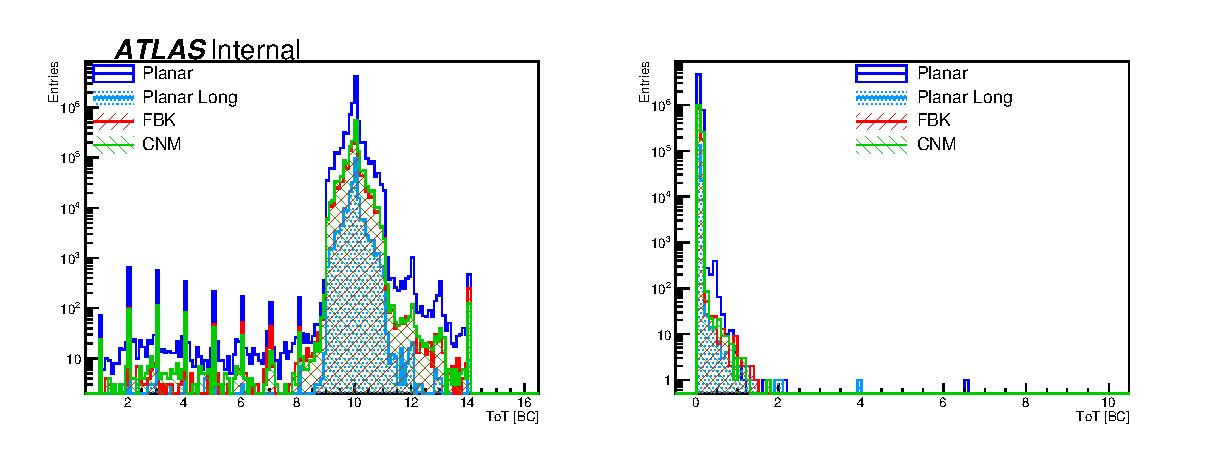
\includegraphics[width=1.\textwidth]{Images/IBL_commissioning/ToTDistro49450.eps}
\caption{ ToT and Sigma of ToT distribution for the IBL detector with an injection charge of 16000e$^-$}
\label{pic:tot_map}
\end{figure}

The control of the ToT is provided by the feedback current of the PreAmp.
When a negative charge is deposited at the input, a positive charge appears at the output of the Preamp.
In an ideal system, the amplitude of this pulse would be $\frac{Q_{in}}{C_{f1}}$, but because of a fast shaping (return to baseline) is required the amplitude will be less. The shorter is the shaping the smaller the pulse amplitude will be with the same charge. the return to baseline is implemented by a feedback system which discharge the capacitor C$_{f1}$ with an almost constant current source.
The negative going pulse at the output of the second stage feeds the negative input of the comparator, with a threshold voltage at the positive input.
The time that the signal will spend over threshold it is then controlled by the feedback current of the PreAmp, which sets the fall time of the preamp output. This can be tuned with a local 4-bit register (FDAC) and 8-bit global register (PrmpVbpf). 
The ToT characterization respect the PreAmp feedback current is shown in Figure~\ref{pic:prmpvbpf} for different value of the local settings. The value of FDAC=30 was chosen as starting point for the entire IBL production.
The method for the ToT calibration was implemented at the production.
During the IBL commissioning a campaign of tuning was performed targeting for a uniform threshold of 2500 electrons and a correspondence of 10 ToT for an injected charge of 16000 electrons, the results of the tuning are shown in Figure~\ref{pic:tot_map}.\\

\begin{figure}
\centering
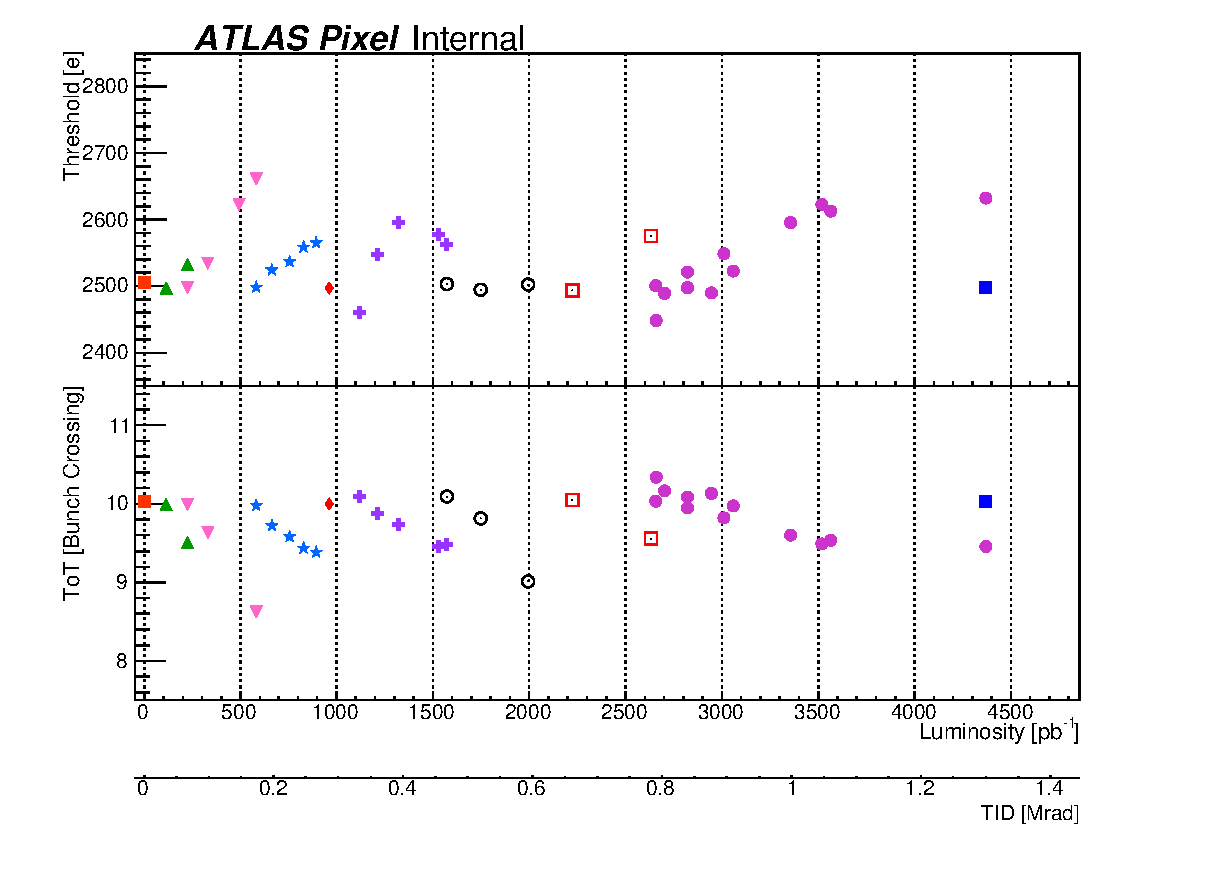
\includegraphics[width=1.\textwidth]{Images/IBL_commissioning/summary_canvas.eps}
\caption{The evolution of the mean threshold and mean ToT measured over all pixels in the IBL detector as a function of the integrated luminosity and the corresponding total ionizing dose (TID) in 2015, as measured in calibration scans. The threshold was tuned to 2500 electrons. Radiation effects caused the measured threshold to drift upward with integrated luminosity, but short periods of annealing and regular re-tunings brought the mean threshold back to the tuning point. Each series corresponds to one tuning.
}
\label{pic:thr_tot_evolution}
\end{figure}
The radiation damage not only affects the sensor performance, but as well, the operation of the several transistor in the FE-I4 chip. In particular the leakage current and the intrinsic threshold of each transistor are affected as described in Chapter 2. The net effect is an influence on the FE-I4 threshold and ToT. The mean threshold of each FE will lower with irradiation and the ToT will increase, as shown in Figure~\ref{pic:thr_tot_evolution}. Given this effect the detector needs to systematically go through the tuning procedure. The effect is expect to saturate after few \SI{}{\mega\radians} of total ionizing dose. At the moment of this thesis tests are on-going to understand the effect in presence of annealing time similar to the one observed during data-taking.\\
%\begin{figure}
%\centering
%\includegraphics[width=0.6\textwidth]{Images/IBL_commissioning/leakage_current.pdf}
%\caption{}
%\end{figure}
%An irradiation campaign was set in place for having a prediction of the phenomenon, the result was a saturation of the leakage current




\subsubsection{Timing optimization}
A tuning of the front-end settings was required to operate the IBL in one bunch-crossing time window.
The data-taking system of the IBL used by a double chip module logic, so it considered a module as composed of 2 front-end chip, regardless the distinction done in the previous chapters. This choice was done for simplifying the data-taking chain, in terms of software and firmware. In the following text such choice will be referred as DAQ module.
The response of each of the front-end needed then to be synchronous with the other front-end in the the same DAQ module. As the data-taking chain cannot apply a correction for a single front-end, the timing adjustment needed to be done at the level of the readout chip electronics itself.
The response quickness of the analog part of the chip can be modified through the discriminator bias, DisVbn, a tunable 8-bit register.
\begin{figure}
\centering
\subfloat[]{\label{fig:disvbn}\includegraphics[width=0.5\textwidth]{Images/IBL_commissioning/ibl_timing_disvbn.png}}
\subfloat[ ]{\label{fig:disvbn_dispersion}\includegraphics[width=0.5\textwidth]{Images/IBL_commissioning/ibl_timing_dispersion.png}}
\caption{\ref{fig:disvbn}~Variation of the latency of front-end chips of a particular module of the IBL as a function of FE-I4 configuration parameter DisVbn to change the discriminator bias.\ref{fig:disvbn_dispersion}~Timing difference between the 2 FEs in the common module of the IBL for the status before the discriminator bias (DisVbn) adjustment and that after the adjustment.}
\end{figure}
Figure~\ref{fig:disvbn} shows the FE latency at the variation of the DisVbn parameter for two readout chip in the same DAQ module. The tuning strategy was then to fix the DisVbn for one of the front-end and to adjust the value for the other chip in order to minimize the latency among the two. The timing difference between two front-end chip in the same DAQ module is shown in~\ref{fig:disvbn_dispersion} before and after the DisVbn adjustment, the maximum time difference for a DAQ module is \SI{4}{\nano\second} after the tuning.

\begin{figure}
\centering
\subfloat[]{\label{fig:ibl_timewalk}\includegraphics[width=0.5\textwidth]{Images/IBL_commissioning/ibl_timewalk.png}}
\subfloat[]{\label{fig:ibl_timing_efficiency}\includegraphics[width=0.5\textwidth]{Images/IBL_commissioning/ibl_timing_eff.png}}\\
\subfloat[]{\label{fig:ibl_timing_final_efficiency}\includegraphics[width=0.5\textwidth]{Images/IBL_commissioning/ibl_final_timing_eff.png}}
\caption{\label{fig:ibl_timewalk}~Timewalk for a single pixel tuned at a threshold of 1485e- and a correspondace of 9 ToT for an injected charge of 16000 electrons. \label{fig:ibl_timing_efficienty}~1 BC In-time efficiency of the IBL as a function of time-over-threshold (ToT) before the timing scan in July 2015 (open circle), and after the timing adjustment (bullet) reflecting the result of the timing scan. The blue histogram is the estimation of the expected efficiency from the result of the timing scan. Note that HitDiscCnfg is set to 0 for the data taking. \label{fig:ibl_timing_final_efficiency}In-time efficiency of the IBL as a function of time-over-threshold (ToT) before (circle) and after (bullet) the tuning at HitDiscCfg=2.}
\end{figure}
The front-end response was not uniform with respect to the charge information, due to time-walk of the analog amplifier in the readout chip. Even if the signal coming from the sensor has usually a rise time of the order of the nano-second, in case of low charge signals the output of the amplifier could take few dozens of nanosecond to reach the threshold of the discriminator. In the case of the FE-I4 this happens for signals just above the threshold of the discriminator. Figure~\ref{fig:ibl_timewalk} shows the time-walk for a single pixel, tuned at 1485 electrons threshold and with a correspondence of 9 ToT for a charge of 16000 electrons; it can be seen that a signal just above threshold require up to \SI{35}{\nano\second} to pass the threshold. This led to a small efficiency in the low ToT regime even after a DisVbn tuning, as shown in Figure~\ref{fig:ibl_timing_efficiency}.
%\begin{figure}
%\centering
%\includegraphics[width=0.5\textwidth]{Images/IBL_commissioning/ibl_final_timing_eff.png}
%\label{fig:ibl_timing_final_efficiency}
%\caption{In-time efficiency of the IBL as a function of time-over-threshold (ToT) before (circle) and after (bullet) the tuning at HitDiscCfg=2.}
%\end{figure}
The FE-I4 can discriminate hits of different sizes in order to associate low ToT hits with the correct bunch crossing in spite of time-walk. This feature is controlled by the HitDiscCnfg register. When HitDiscCnfg is set to zero, this disables any small/large hit discrimination and any time the comparator fires this is counted as a hit occurring at in the bunch crossing that the comparator fires. As Figure~\ref{fig:ibl_timewalk} shows, for hits close to the threshold the firing of the comparator is delayed due to time-wals and therefore such hits will appear in the wrong bunch crossing. Setting the HitDiscCnfg to 1 (2) means that only hits with ToT greater than 1 (2) clocks are counted as stand-alone hits in the bunch crossing the the comparator fires, those hits are called "big hits". Because big hits are significantly above threshold, they are hardly affected by time-walk and so they appear in the correct bunch crossing. Hits with TOT less than 1 (2), called small hits, are only discarded if they occur in isolation (no other hits in their vicinity). Otherwise, small hits are counted in the same bunch crossing as any neighbor big hits, within an association window 2 bunch cross wide.
Figure~\ref{fig:ibl_timing_efficiency} shows the efficiency for different ToT values. Two situation are considered, HitDiscCnfg set as 0, for which the small hit efficiency is very low, and HitDiscCfg set as 2, for which the small hit efficiency is above 90\percent. The test were performed in different period, and at the time of the test with HitDiscCnfg = 2 there were also improvement in the transmission line fine delay setting that led to an improvement in the efficiency even for ToT$ \ge 3$.

\subsection{The IBL mechanical stability}
During the commissioning and alignment of the IBL using cosmic-ray data, a mechanical distortion of the IBL was observed. This distortion is caused by a difference in the coefficients of thermal expansion of the IBL stave components. 
\begin{figure}
\subfloat[\label{fig:ibl_bowing_full_package}]{\includegraphics[width=0.49\textwidth]{Images/IBL_commissioning/ibl_bowing_fullpackage.png}}
\subfloat[\label{fig:ibl_bowing_one_stave}]{\includegraphics[width=0.49\textwidth]{Images/IBL_commissioning/ibl_bowing_onestave.png}}
\caption{\ref{fig:ibl_bowing_full_package} Full package of the IBL staves with the central ring simulated by the 3D FEA representing the distortion.
The size of the distortion is magnified for visualization. The color represents the relative size of the local
displacement. The temperature is set at T = \SI{-60}{\kelvin} uniformly from the nominal temperature. The distortion
is magnified by factor 20. \ref{fig:ibl_bowing_one_stave} Visualization of the distorted stave with magnified distortion size. The size of the
distortion is magnified for visualization. The color represents the magnitude of the displacement. The right bottom
graph shows the relative displacement size in local-x direction as a function of the global z-position at the face plate surface of the stave.}


\label{fig:ibl_bowing_staves}

\end{figure}
A three-dimensional finite element analysis (FEA) is performed to understand the observed large distortion of the IBL staves \cite{ibl_bowing_1}. The model is 14-fold symmetric around the beam pipe and considers the detailed structure of the staves. The FEA implements the constraint due to the central ring and mechanical boundary conditions at screws, alignment pins and
glues. A uniform temperature is assumed over the full package of the IBL in calculation of the distortion
in this simulation.
The FEA simulation shows that the stave bows to the negative direction in the ATLAS global coordinate
system when it is cooled down (Figure \ref{ibl_bowing_staves}). The CTE of the bare stave is almost zero ppm, while the
polyimyde flex bus line (Stave Flex) glued on one side of the bare stave is several tens of ppm. The Stave Flex shrinks more than the bare stave, resulting in the bowing of the stave, towards
the azimuthal direction. The FEA simulation also predicts radial distortions other than the region around
the central ring.
The FEA simulation calculates that the magnitude of the bowing is expected to be approximately parabolic
to the azimuthal direction with maximum at the center of the stave (Figure \ref{fig:ibl_bowing_one_stave}). At T =\SI{-60}{\celsius}.
from the nominal temperature the magnitude of the displacement is calculated to be about $0.27 \milli \meter$
at the center of the stave. 

\subsubsection{Measurement of the bowing and thermal stability}
In order to study the temperature correlation to the size of the IBL distortion, cosmic-ray events were
collected in March 2015 at different temperature set points: $+15 ^{\circ} C \rightarrow +7 ^{\circ}C \rightarrow 0^{\circ}C \rightarrow -10 ^{\circ}C \rightarrow -15 ^{\circ}C \rightarrow -20 ^{\circ}C$. To quantify the size of the IBL distortion, track-based alignment corrections \cite{ibl_dist_4} are applied to determine the positions of the IBL modules as well as their geometrical distortions relative to
the nominal (ideal simulated) geometry.
There are more than 5$\times 10^5$ events of cosmic-ray data accumulated at each temperature set point with
both the toroid field and the solenoid field on. The trigger for cosmic-ray events is the Fast-OR trigger of
the Transition Radiation Tracker (TRT), a hardware-based logical OR of the TRT wires having a hit along
a likely muon track path. The trigger efficiency is over 90\percent \cite{ibl_dist5} and an average rate of \SI{4.84}{\hertz}. Tracks are reconstructed from hits measured by three subdetectors: the Pixel Detector (including the IBL), the
Semiconductor Tracker (SCT), and TRT. 17\percent of Fast-OR triggered events were used in the distortion
studies after a series of track quality cuts:
\begin{itemize}
\item $N_{Pixel} + N_{SCT} \ge 
4$: at least four silicon hits;
\item $N_{TRT} \ge 
25$: at least 25 hits in the TRT;
\item $\pt^{trk} \ge 2 GeV$: 2 GeV threshold of the transverse momentum.
\end{itemize}
The $\pt^{trk}\ge 2 GeV$ is applied in order to reduce the impact of multiple scattering in the traversed
material.
The unbiased track-to-hit residual vector, $\vv{r}_{res} = \vv{r}_{hit} - \vv{r}_{exp}$, is used to quantify the distortion of the IBL,
where $\vv{r}_{hit}$ is the vector of measurements of the hit position in the module and $\vv{r}_{exp}$ is the expected position
according to the track fitting. Both are defined in the local coordinate system \footnote{In the IBL module frame, the x and y axes are defined in the detector plane with the x-axis pointing along the most precise
measurement direction. The x-axis is orientated along the transverse plane in the ATLAS coordinate system. The y-axis is
pointed along the beam direction.} of the module registering
the hit. Residuals are defined as unbiased, when the hits on a certain module are removed from the track fit before computing the track-to-hit residual.
To demonstrate the distortion effect due to temperature variation, a set of initial alignment constants with
ideal geometry of flat staves is used as the reference constant set for the track reconstruction. There is a
global alignment for the whole IBL as a rigid body to account for global displacement of the IBL with
respect to the other ID sub-detectors. There are total 3 degrees of translation and 3 degrees of rotation for
the IBL. This initial alignment corrections \cite{ibl_bowing_4} is derived from the cosmic-ray data collected in February 2015. 
\begin{figure}
\subfloat[\label{fig:ibl_bowing_Xresidual}]{\includegraphics[width=0.49\textwidth]{Images/IBL_commissioning/ibl_Xresidual_AfterAlignment.png}}
\subfloat[\label{fig:ibl_bowing_Yresidual}]{\includegraphics[width=0.49\textwidth]{Images/IBL_commissioning/ibl_Yresidual_AfterAlignment.png}}
\caption{The track-to-hit residual mean in the (a) local-x and (b) the local-y direction. The residual mean is
averaged over all hits of modules at the same global-z positon. The alignment corrections derived at $-20^{\circ}C$ are
applied to the local positions in the module frames. For local-x, each data set is fitted to a parabola which is
constrained to match to the baseline B = 0 at z = z0 = 3
66.5 mm.}
\label{fig:ibl_bowing_residual}
\end{figure}
Using cosmic-ray data collected in March 2015, the magnitude of the distortion
is found to depend linearly on the operating temperature of the IBL, with a gradient of
 $10 \micro \meter /K $.
In order to quantitatively estimate the temperature gradient, a set of module level alignment correction
was calculated using the data collected at $-20^{\circ}C$. The module level alignment takes each individual IBL
module as the basic element of the geometry correction. Three degrees of translations, and one degree
of rotations around local-z axis are allowed. The
observed residual after this alignment correction at $-20^{\circ}C$ in the Figure \ref{fig:ibl_bowing_residual} is consistent with zero, which
shows that the distortion of the IBL can be corrected with the alignment algorithm. The y-residual shows
no temperature dependence effect within $20 \micro \meter$ uncertainty.
The FEA simulation calculates that the averaged local-x residuals $x_L$, is
expected to be parabolic. Therefore a fitting function to describe $x_L$, is parametrized with the following
parabolic function:
\begin{equation}
\Delta x_L(z) = B- \frac{M}{z^2_0}(z^2-z^2_0)
\end{equation}
where $z$ is the global $z$ position of the module, $z_0 = 366.5 \milli \meter$ is the fixing point of the stave at both ends,
$B$ is the baseline which describes the overall translation of the whole stave and $M$ is the magnitude of
the distortion at the center of the stave. $B$ is set to a common constant for all temperature points because
the end-blocks of each stave are fixed mechanically. M is the free parameter in the fit and it can be used
to quantify the size of the distortion. The parametrization function describes distortion shape of each
temperature as presented in Figure \ref{fig:ibl_bowing_Xresidual}
\begin{figure}
\centering
\includegraphics[width=0.5\textwidth]{Images/IBL_commissioning/ibl_distorsion_magnitude.png}
\caption{The magnitude of the distortion as a function of the temperature set point. Each data point is a best fit of a
parabola to the local-x residual mean as function of the global-z of the module position. The alignment corrections
derived at $-20^{\circ}C$ are applied to the local positions in the module frames.}
%the local positions in the module frames.}
\label{fig:ibl_bowing_magnitude}
\end{figure}
Figure \ref{fig:ibl_bowing_magnitude} shows the magnitude of the distortion as function the operating temperature. A linear dependence
on operating temperature of the magnitude of the distortion is observed. The temperature gradient of the
magnitude of the distortion, M, is fit as:
\begin{equation}
\frac{dM}{dT} = -10.6 \pm 0.7 [\micro \meter /K]
\end{equation}
The uncertainty on the above gradient is estimated by comparing to a fit performed without constraining
the baseline B in addition to the statistical uncertainty. The observation supports the hypothesis that the
distortion is driven by the mismatch of the coefficient of thermal expansion.
For a correct operation of the IBL detector a stable temperature is therefore required. The sources of temperature instability are the intrinsic stability of the cooling system as well as the environment and the variation in power consumption of the front-end modules.
Since the thermal capacity of the cooling system is much larger than the module?s power consumption,
the cooling pipe temperature stability is assumed to be decoupled from the variation of the power consumption.
The stability of the temperature of the IBL cooling system was investigated using the temperature sensor
monitoring system during the same cosmic-ray run studied in the previous section. There are 10 negative
temperature coefficient (NTC) thermistors for each stave. They are composed of one NTC for every four
front-end chips (eight in total per stave) and one NTC for each of the inlet and outlet sides of the cooling
pipe at $z \simeq \pm 700 \milli \meter$. The precision of the NTC sensors on modules and the sensors on the cooling pipe
is estimated to be $\sim 0.02 K$. The IBL employs a bi-phase CO2 cooling system \cite{ibl_bowing_6}. The coolant, CO2,
is liquid at the inlet and it transits to bi-phase (gas and liquid) as it absorbs the heat dissipated in the stave.
The actual position of transition varies by staves. Therefore the outlet side is considered to represent the
temperature of the coolant temperature reference more accurate than the inlet side. On the other hand, the
NTC sensors on modules are used to evaluate the temperature stability at the modules.
For each sensor $i$ of each run $k$, the temperature value is read out $N^{(k)}_i$ times in the detector control system, while each run is a block of the data-taking period. The standard deviation and the peak-to-peak values
of each sensor i of each run k are defined as:
\begin{equation}
\begin{array}{l}
\text{Standard deviation:}\quad \delta T^{(k)_i} = \sqrt{\frac{1}{N^{(k)}_i} \sum_{j} (T^{(k)}_i[j]-<T^{(k)}_i>)^2}\\
\text{Peak to peak:}\quad \Delta T^{(k)}_i = max_{(j)}(T^{(k)}_i[j]) - min_{(j)}(T^{(k)}_i[j]).
\end{array}
\end{equation}
where $T^{(k)}_i[j])$ is each temperature readout and $<T^{(k)}_i>$ represents the average temperature readout.
For the cooling pipe outlet, there are 14 sensors in total. The standard deviation of $\delta T^{(k)}_i[j]$ over 14 sensors, denoted as:
\begin{equation}
\delta(\delta T^{(k)}) = \sqrt{\frac{1}{14} \sum_i {(\delta T^{(k)}_i - <\delta T^{(k)}>)^2}},
\end{equation}
where $<\delta T^{(k)}>$ represents the average of $\delta T^{(k)}_i$ over 14 sensors.
\begin{figure}
\centering
\subfloat[\label{fig:rms_cool}]{\includegraphics[width=0.7\textwidth]{Images/IBL_commissioning/AvgRMScool.pdf}}\\
\subfloat[\label{fig:rms}]{\includegraphics[width=0.7\textwidth]{Images/IBL_commissioning/AvgRMS.pdf}}
\caption{Stability of the outlet of the cooling pipe (a) temperature and module (b) temperature sensors of the IBL during the comic-ray data-taking in the commissioning phase. Each bar represents the block of data taking period called runs. The width of each bar represents the duration of the data-taking of the run. For each module temperature sensor, the RMS and the peak-to-peak values
of the temperature readout during the run are calculated. The ?RMS? bar in the figure represents the variance of the
RMS values of the 112 temperature sensors with indicating $\pm 1$ RMS range around the average RMS. The ?peaktopeak? bar represents the variance of the peak-to-peak values of the 112 temperature sensors with indicating the maximum and the minimum peak-to-peak values among the 112 temperature sensors.}
\end{figure}
Figure \ref{fig:rms_cool} shows the results of the stability study using the cooling outlet pipe temperature sensors. Each bar represents a run. There are two kinds of
bars denoted as ?RMS? and ?peak-to-peak?. The vertical range of the RMS bar for each run k is defined
as:
\begin{equation}
\text{RMS:}\quad[<\delta T^{(k)}> - \delta(\delta T^{(k)}), <\delta T^{(k)}> + \delta(\delta T^{(k)})],
\end{equation}
and the vertical range of the peak-to-peak bar is defined as:
\begin{equation}
\text{peak to peak:}\quad[min_{i}(\Delta T^{(k)}_i), max_{i}(\Delta T^{(k)}_i)].
\end{equation}
The width of each bar represents the duration of the corresponding run. As seen in the plot, the RMS bar
of the temperature during a run is well within $0.05 K$ while the peak-to-peak bar is within $0.2 K$.
The same summarization of the stability is performed for 112 NTC sensors on the modules, and the result
is shown in Figure \ref{fig:rms}. For most of the runs the peak-to-peak value of them are within $0.25 K$, which is
not significantly larger than the stability of the outlet cooling pipe of $0.2 K$. The maximum peak-to-peak
values in some of the runs are close to $0.4 K$. These excess values are recorded by the sensors which are
the closest to the inlet cooling pipe. It is considered that the temperature fluctuation at this position is
caused by the bi-phase transition of the CO2 coolant. Such a local temperature fluctuation is expected to
have small impact to the global distortion of the stave. The fact that the variation of module temperature
is not very deviated from the cooling output pipe temperature stability indicates that the dominant source
of the module temperature variation could be considered to be from the stability of the cooling system
and environment.

\subsubsection{Effect on the performance}
In order to assess the effect of track reconstruction under varying temperature conditions, a set of alignment
constants is produced to mimic the IBL stave distortion in the local-x axis. It is assumed that
a certain amount of displacement of module positions, generated by the temperature fluctuation under
stable collision data-taking, is not corrected by the alignment procedure.
The magnitude of the distortion is calculated for a $\delta T_{flex} = \SI{0.2}{\kelvin}$, corresponding to $2\micro \meter$ displacement at the center of the stave.
It is expected that the transverse impact parameter (d$_0$) of a charged track is the most sensitive track
parameter to the distortion of the IBL.
\begin{figure}
\centering
\includegraphics[width=0.5\textwidth]{Images/IBL_commissioning/ibl_d0effect.png}
\caption{Distribution of the transverse impact parameter d$_0$ of charged tracks with respect to the beamspot from Z$\rightarrow \mu^+ \mu ^-$ events simulated in $\sqrt{s}= \SI{13}{\TeV}$ proton-proton collisions. Solid Circle shows the nominal geometry and the open square the distorted geometry corresponding to a temperature variation of the IBL of $\delta$ T$_{flex} = \SI{0.2}{\kelvin}$ (\SI{2}{\micro \meter} displacement at the center of the stave)}
\label{fig:d0effect}
\end{figure}
Figure~\ref{fig:d0effect} shows the d$_0$ distribution of muon charged tracks with respect to the beamspot using the MonteCarlo simulation of Z$\rightarrow \mu^+ \mu ^-$ events in $\sqrt{s}= \SI{13}{\TeV}$ proton-proton collisions based on the nominal geometry and the distorted geometry. For each event, only a pair of opposite sign reconstructed muons with the invariant mass of 60<m$_{\mu \mu}$<120 GeV, and with the opening angle of two muons greater than 0.2 radians is selected. The track quality selection is similar to the one used for the alignment except for the minimale threshold of the transverse momentum, increased to 15 GeV.
The bias to the transverse impact parameter (d$_0$) is $\sim \SI{1}{\micro \meter}$, small in comparison to the expected $d_0$ resolution, O(\SI{10}{\micro \meter}).\\
\begin{figure}
\subfloat[\label{fig:bowing_ROC}]{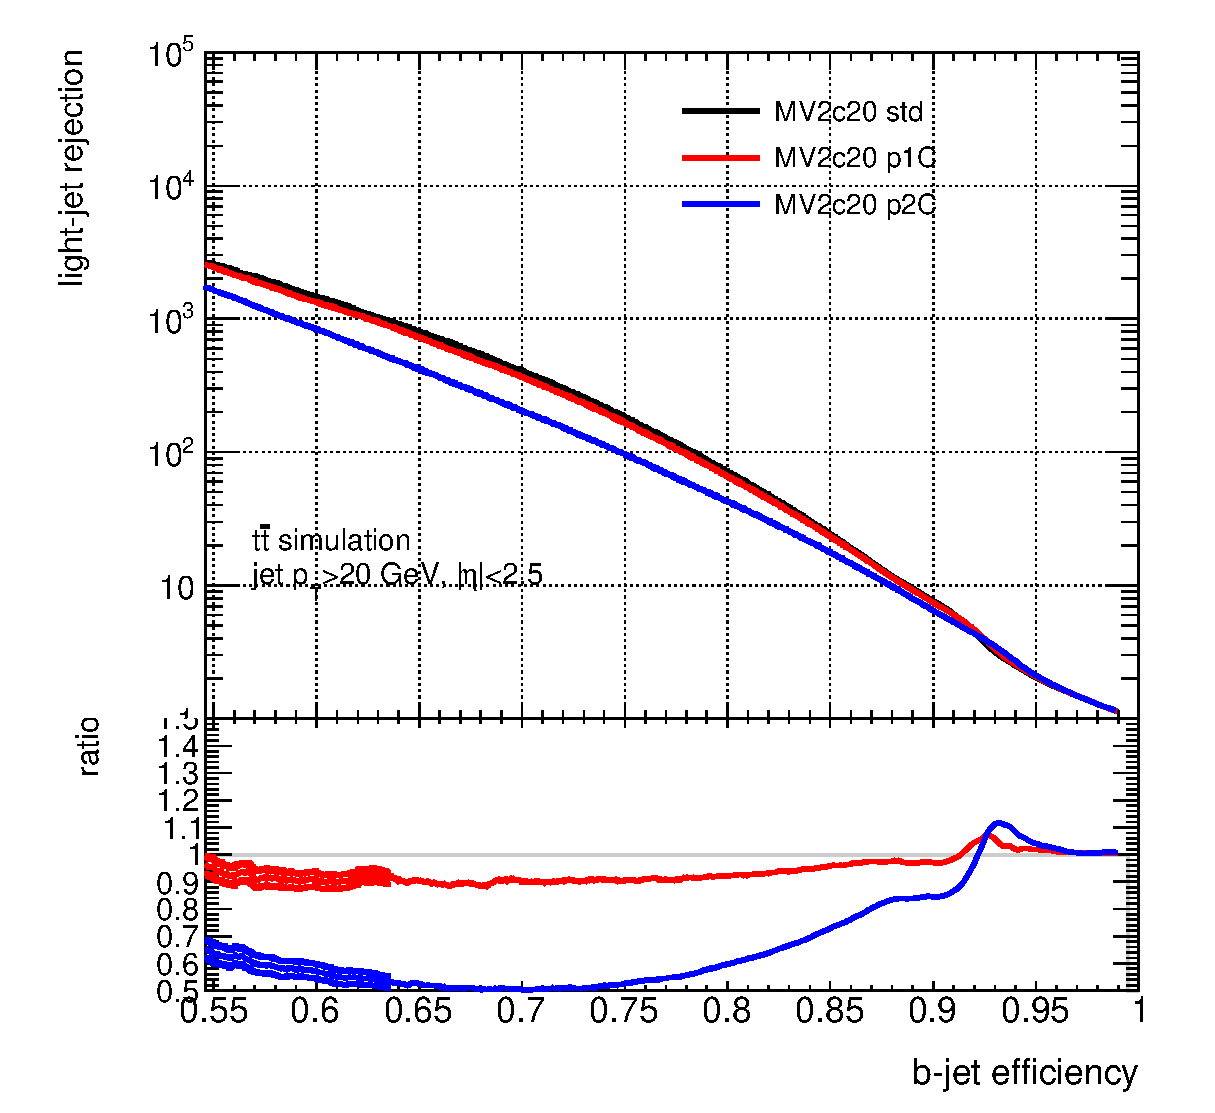
\includegraphics[width=0.5\textwidth]{Images/IBL_commissioning/bVSlight__MV2c20.eps}}
\subfloat[\label{fig:bowing_flat}]{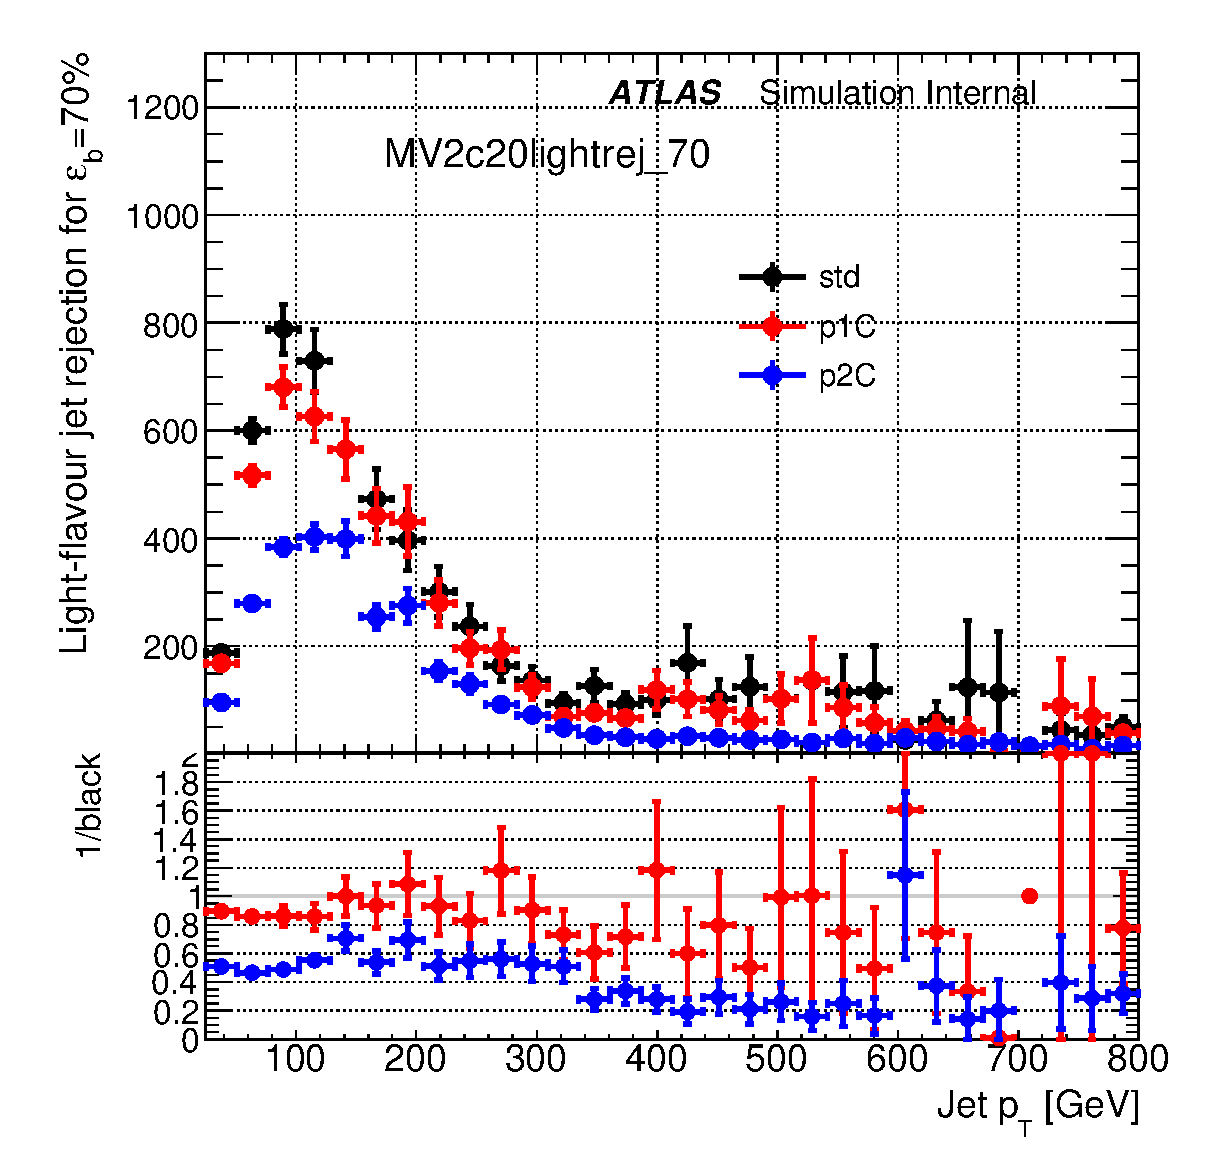
\includegraphics[width=0.5\textwidth]{Images/IBL_commissioning/MV2c20lightrej_70__jet_pt___flat.eps}}
\caption{Light-jet rejection evaluated with the MV2c20 algorithm with respect to b-tagging efficiency \subref{fig:bowing_ROC} and in function of jet-\pt for a nominal b-tagging efficiency of 70\% . Three different bowing scenarios are shown; the nominal geometry and the foreseen effect for a temperature stability of 1K and 2K. For 1K (2K) temperature stability the mechanical stability is expected to be \SI{1}{\micro\meter}(\SI{2}{\micro\meter}) }
\end{figure}
Further investigations were performed to assess the impact on b-tagging performance for different scenario, with a $\delta$T$_{flex} = \SI{0.2}{\kelvin}, \SI{0.5}{\kelvin}, \SI{1}{\kelvin}, \SI{2}{\kelvin}$, in the MonteCarlo simulation of t$\overline{t}$ events in $\sqrt{s} = \SI{13}{\TeV}$. In the case of $\delta T_{flex} = \SI{0.2}{\kelvin}, \SI{0.5}{\kelvin}$ b-tagging performance do not deteriorate. An impact in b-tagging performance was observed for $\delta T_{flex} = \SI{1}{\kelvin}$ and \SI{2}{\kelvin}, as shown in Figure~\ref{fig:bowing_ROC}, with light-jet rejection decrease respectively to the 90\percent and the 50\percent of the nominal value for a 70\percent b-tagging efficiency working point. Figure~\ref{fig:bowing_flat} shows the light-jet rejection at 70\percent b-tagging efficiency working point in function of the Jet-\pt. The higher the Jet-\pt is, the more tracks are collimated. As it will be explained in Chapter 7, for high-\pt  jet is crucial a good reconstruction of the impact parameter significances ($\frac{d_0}{\sigma_{d0}}$ and $\frac{z_0}{\sigma_{z0}}$). At \pt higher than 300 \GeV (high-\pt) tracks within a jet are more collimated than in the low-\pt  case, so the impact parameter is usually lower. On the other side the multiple scattering contribution to the error is less significant, so that the impact parameter significance is mostly biased by the systematic
so that the effect of the bowing affects more the b-tagging performance. This can be seen in the fact that for the \SI{2}{\kelvin} scenario and jet with \pt higher than \SI{350}{\GeV} the light-jet rejection is just the 30\percent of the default case. \\

\subsection{Measurement of the Lorentz angle}
During the cosmic data-taking phase, occurred in the commissioning of the ATLAS detector, a study of the silicon detector properties was carried out. In particular a measurement of the Lorentz angle was putted in place.\\
%In absence of magnetic field, charge carriers drift inside the silicon bulk following the electric field generated by the bias voltage which is perpendicular to sensor plane in planar sensors and parallel to it in 3D sensors.
As described in Chapter 1, the Inner Detector operates in a constant magnetic field of \SI{2}{\tesla} generated by the ATLAS solenoid magnet. 
The presence of magnetic field has to be considered for the study of the electron/hole pairs drift in the silicon bulk, as introduced in Chapter 2, with the concept of the Lorentz angle.\\
For IBL two different technologies of silicon sensors have been used, the Planar and the 3D. As previously said the main difference of the two technology is the geometry of electrodes and the consequent orientation of the electric field. In Planar devices the electric field is perpendicular to the solenoidal magnetic field and so the Lorentz mechanism is present. In 3D technology, instead, the electric field is parallel to the magnetic field and the effect of the Lorentz force is null.\\


\begin{figure}
\centering
\includegraphics[width=0.5\textwidth]{Images/IBL_commissioning/lorentz_angle.png}
\caption{Variation of the mean cluster transverse width with transverse incidence angle for pixel layers and IBL sensors. }
\label{pic:IBL_lorentz}

\end{figure}

This is what can be seen in Figure~\ref{pic:IBL_lorentz} which shows the average transverse dimension of the clusters as a function of $\phi_{inc}$ for the IBL sensors and the ones used in the other 3 layer of the Pixel Barrel Detector. In planar sensors, the minimal cluster width is reached when the particle incidence angle coincides with the drift angle of the charge carriers. This angle is called the Lorentz angle and is a property of the silicon bulk for a given magnetic field. We can see that pixel layers and IBL planar have their minimum in the same region, while 3D sensors are compatible with the expected zero value of the Lorentz angle.\\

The curve can be fitted with the following function of incident angle $\alpha$:
\begin{equation}
F(\alpha) = [a (\tan \phi_{inc} - \tan \alpha_L) + \frac{b}{\sqrt{\cos \phi_{inc}}}] \otimes G(\phi_{inc})
\end{equation}

where $\otimes$ indicates the convolution operator and G is the Gaussian function. The free parameters of the fit are the values of a and b, the standard deviation of the Gaussian, and the Lorentz angle value $\alpha_L$.
In the formula, the term $a (\tan \phi_{inc} - \tan \alpha_L)$ represents the geometrical projection of the charge carriers liberated by the particle on the sensor surface. The parameter a varies with how rapidly the cluster size increases with the incident angle. The term $\frac{b}{\sqrt{\cos \phi_{inc}}}$ describes the cluster size, where b is the mean cluster size for tracks at the Lorentz angle. Fit results are shown in the Table~\ref{tab:fit_Lorentz}.
\begin{table}
\centering
\begin{tabular}{|c|c|c|c|c|c|}
\hline
Technology & a[pixels] & $\alpha_L$[\SI{}{\milli\radians}] & b[pixels] & $\sigma$ [\SI{}{\milli\radians}] & $\chi^2$/d.o.f \\
\hline
Pixel Layers & 3.28\pm0.02 & 201\pm1 & 1.14\pm0.01 & 80\pm4 & 64/23 \\
IBL Planar & 2.35\pm0.06 & 224\pm4 & 1.18\pm0.03 & 112\pm21 & 41/23 \\
Pixel Layers & 2.90\pm0.07 & -10\pm5 & 1.08\pm0.03 & 64\pm20 & 19/23 \\
\hline
\end{tabular}

\caption{Lorentz angle fit for the three sensor technologies of the Pixel Detector with cosmic data in 2014. Errors are statistical only.}
\label{tab:fit_Lorentz}
\end{table}
The a parameter varies as expected with the sensor thickness, while the minimal cluster size (b) is obtained for 3D sensor, confirming the small amount of charge sharing at normal incidence in this technology.
The deviation from 0 of the 3D Lorentz angle (\SI{10}{\milli\radians}) can be considered as a fair estimation of the systematic error on the Lorentz angle. This error includes temperature difference between modules, track and cluster selection, cluster position estimation, alignment uncertainty and fit range. More statistics are needed to study separately each of these sources.
\pagebreak
